\chapter{Mankiw微观经济学笔记}

\section{经济学十大原理}

\subsection*{人们面临权衡取舍}

最常见的取舍在于对资源的分配, 另一种取舍在于如何平衡效率(社会能从稀缺资源中得到最大利益)与平等(经济成果在社会成员中平均分配). 

\subsection*{机会成本原理}

机会成本, 即为了得到某种东西而必须放弃的东西. 用粗糙的数学视角来看, 就是说在选择$A_1,\cdots ,A_n$之间存在一个关联$f$, 使得$f(A_1,\cdots ,A_n)$为定值$0$. 

\begin{example}{生产可能性边界}
	考虑一个电脑-汽车生产的模型. 在这个模型中, 让生产电脑的工人转而生产汽车, 将会导致汽车产量增加和电脑产量下降, 反之亦然. 因此, 我们可以用电脑产量作为机会成本来描述汽车产量. 
	\begin{figure}[H]
		\centering
		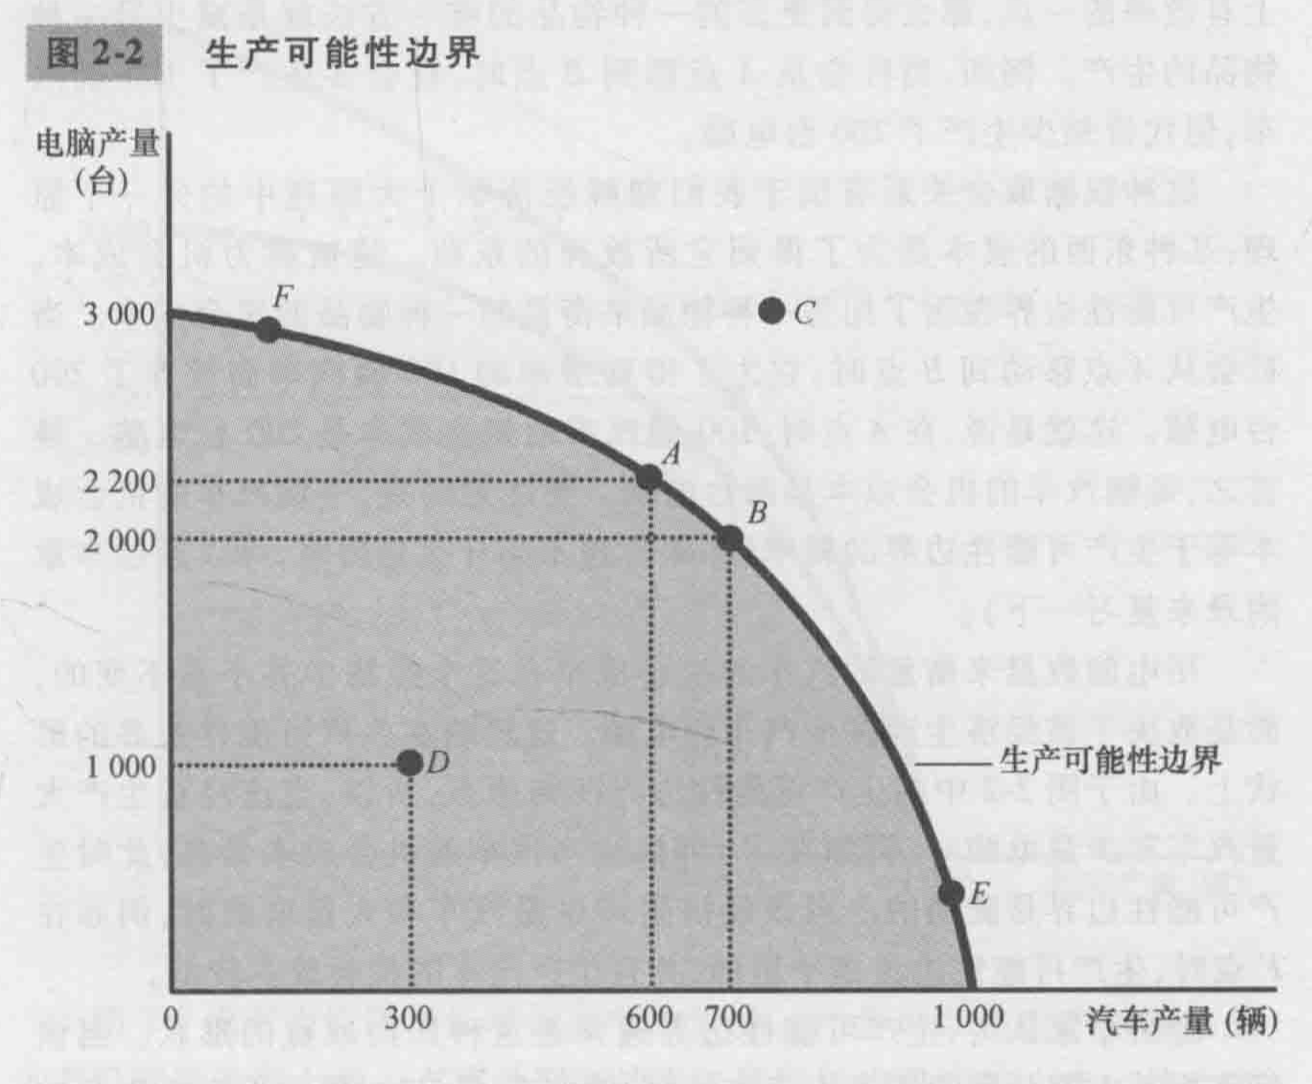
\includegraphics[width=8cm]{attachment/Fig2_2.png}
	\end{figure}
	从数学的视角来看, 两种产量$A_1,A_2$具有类似$A_1+A_2=C$的关系. 特别地, 极端追求汽车产量会让大量熟练于电脑生产的工人转而生产汽车, 这时付出很多电脑工人也只能推动汽车产量的微小变化, 因此越靠近$E$点, 一单位汽车所对应的电脑成本越高. 即是说整个曲线呈现上凸的形状. 
\end{example}

\subsection*{理性人考虑边际量}

实际上, 这个原理基于某种公设, 即所谓理性人(经济人)假设: \textit{人们总是以理性和利己的行为追求目标利益最大化}. 

用数学的话, 考虑一个将行为变成结果的函数$f$. 为了让$f(x)$取得最大值$M$, 可以先找到那些使得$f(x)$与$M$差距不大的$x$, 再在这些$x$(边际量)中找到$f(x)=M$的点. 

\begin{example}{沉没成本}
	已经付出且不可收回的成本, 就成为沉没成本. 按照边际分析的原理, 理性人不应当考虑沉没成本, 因为此时再付出多少都与沉没成本无关. (当然这是在不考虑个人情绪价值等的情况下)
\end{example}

\subsection*{人们会对激励做出反应}

在分析经济行为的后果时, 不仅要考虑其本身直接后果, 还要考虑其作为激励的影响. 

\begin{example}{关于弹性的直观认知}
	提高价格的确能增加生产者的单件收入, 但这会导致消费者的购买量减少, 总收益不一定增加. 实际上, 当需求弹性较小时收益会增加. 
\end{example}

\subsection*{比较优势原理: 贸易可以使每个人的状况都变得更好}

当贸易的两者各具有一方面的特长时, 贸易的优势是显然的. 实际上, 当其中一者具有绝对性优势时, 贸易也会带来改善. 例如, 回到例1.1的情景, 如果两个工厂$A_1,A_2$都开设电脑-汽车的生产线, 即使$A_2$的生产可能性边界较$A_1$更向外(即具有两方面的优势), 在它们之间必有其一生产汽车的机会成本更小, 同时(因为只有两种产物)其生产电脑的机会成本更大. 

因此, 贸易可以让每个人都从事自己最擅长(具有比较优势)的活动, 从而改善所有人的状况. 

\subsection*{市场通常是组织经济活动的好方法}

在后面我们会分析, 利用市场达到供给-需求均衡, 会使市场总收益最大化. 

\subsection*{政府有时可以改善市场结果}

政府需要保证市场的正常开展、避免或补救市场失灵(市场本身无法有效配置资源, 例如出现垄断、发生灾害等)、保证某种平等. 

\subsection*{一国的生活水平取决于它生产物品与服务的能力}

\subsection*{当政府发行了过多货币时, 物价上升}

\subsection*{社会面临通货膨胀与失业之间的短期权衡取舍}

\newpage
\section{分析市场运行的基本工具}

所谓市场, 即是由某种物品或服务的买者和卖者组成的一个群体. 为了构建理想化的模型, 我们总是考虑\textit{(完全)竞争市场}: 买者和卖者的数量足够多、商品之间的差异足够小以至于每个人对价格的影响都是微乎其微的. 之后会介绍如何在完全竞争市场模型的基础上进行针对税收、垄断等的分析. 

\subsection{需求与供给}

1. \textit{需求量}: 买者愿意并且能够购买的一种物品的数量. 在考虑需求对价格的反应时, 人们一般会在价格上升时减少自己的需求量(前提是这种物品的需求量随收入增加而增大; 这被称作\textit{需求定理}). 我们可以用大致的线性关系图像来表达这一定理. 其中, 随着价格的变化而改变的需求量称作\textit{在曲线上的移动}, 不同于\textit{将整个曲线进行移动}. 这意味着我们总有两种方式改变需求量: 变动价格或给予激励. 

\begin{figure}[H]
	\centering
	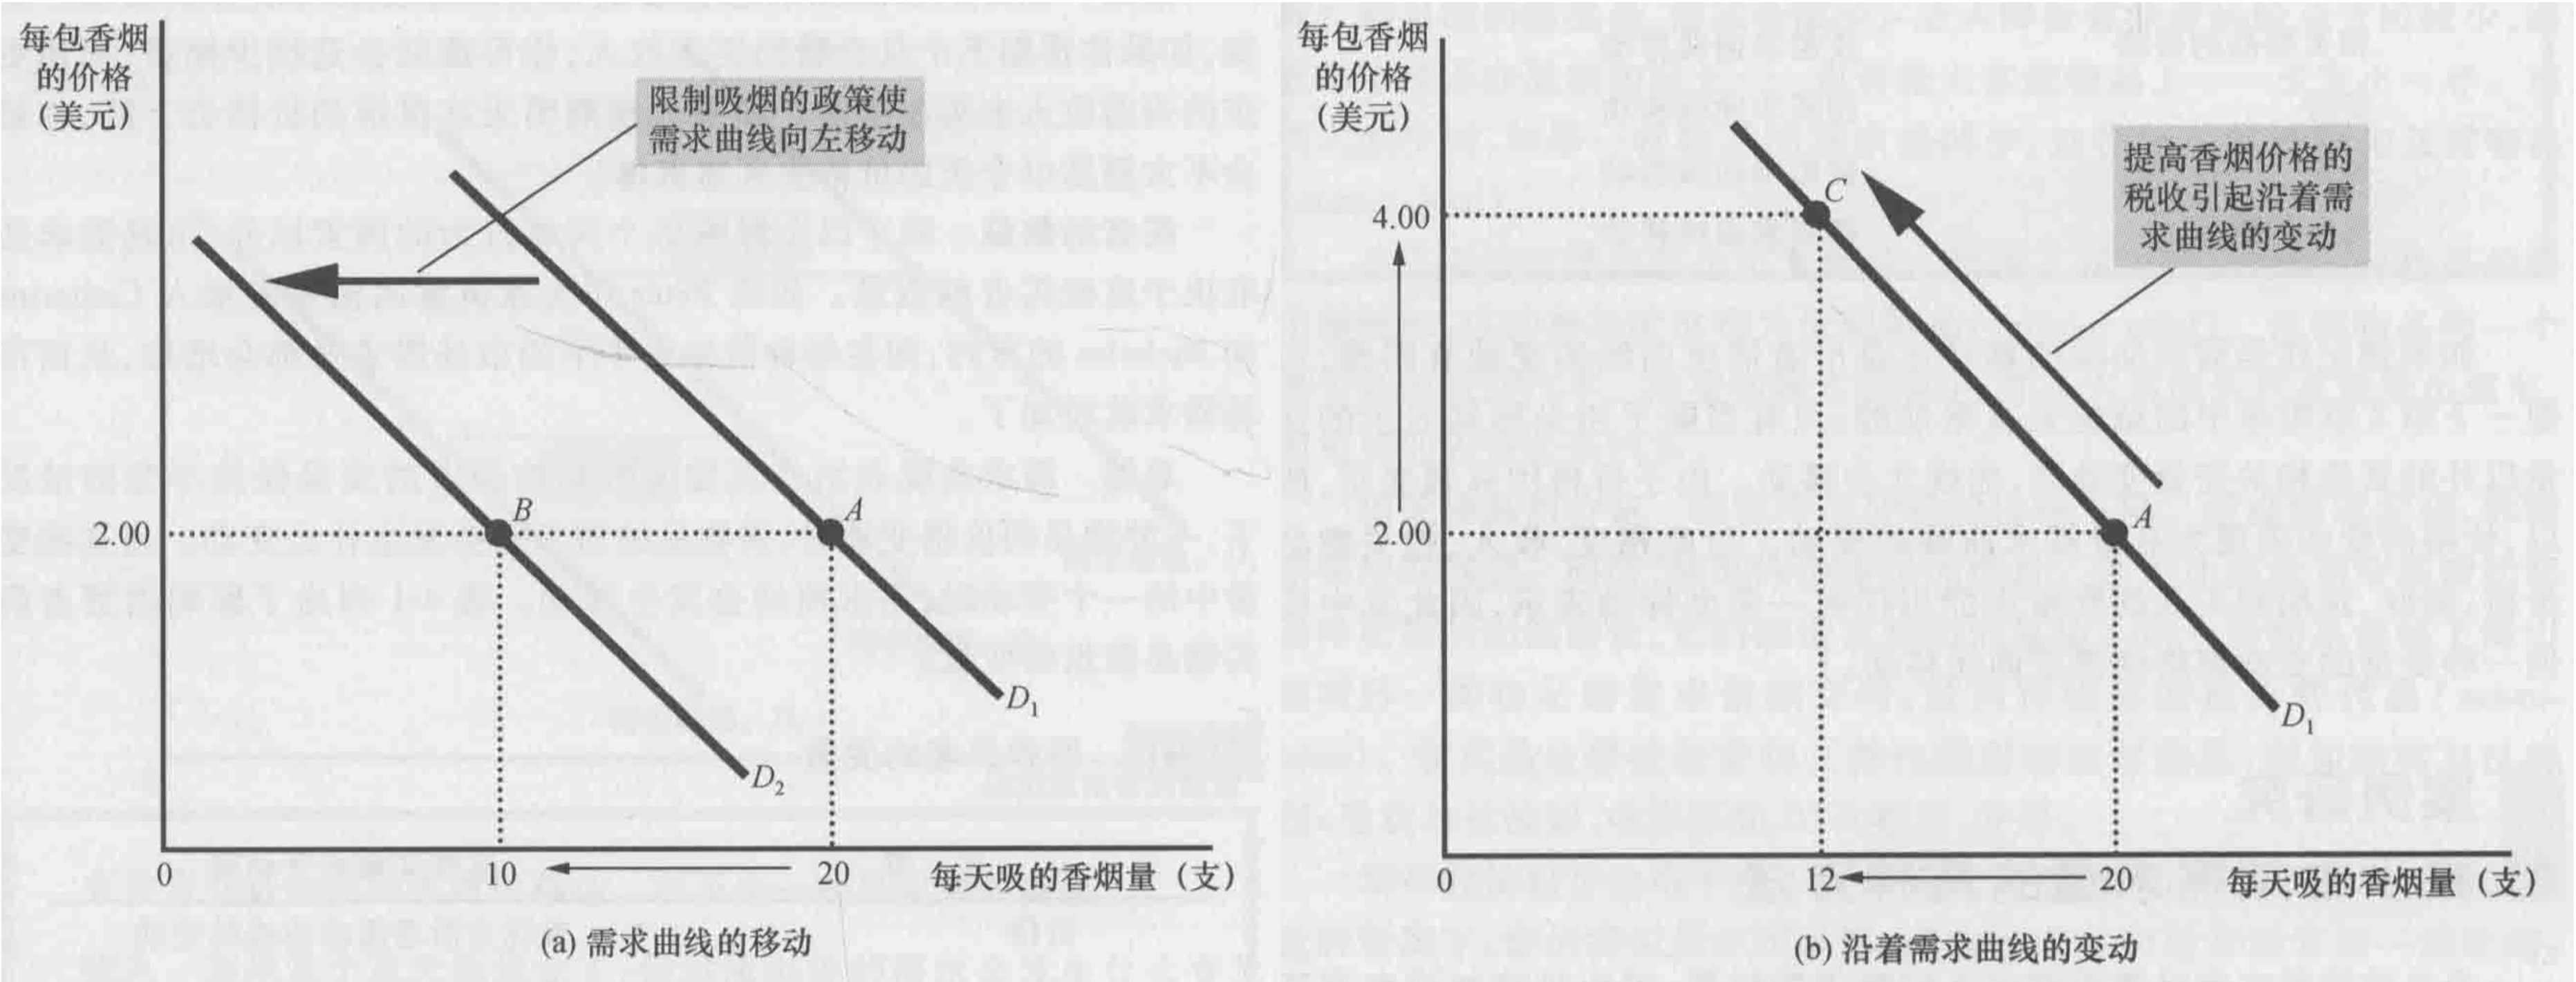
\includegraphics[width=18cm]{attachment/Fig4_2.png}
\end{figure}

与需求曲线移动相关的量: 收入(高档物品, 低档物品), 相关物品的价格(替代品, 互补品), 偏好, 预期, 相关激励等等. 

2. \textit{供给量}: 卖者愿意并且能够出售的该种物品的数量. 类似于需求, 我们有\textit{供给定理}: 一种物品价格上升, 其供给量增加. 

\begin{figure}[H]
	\centering
	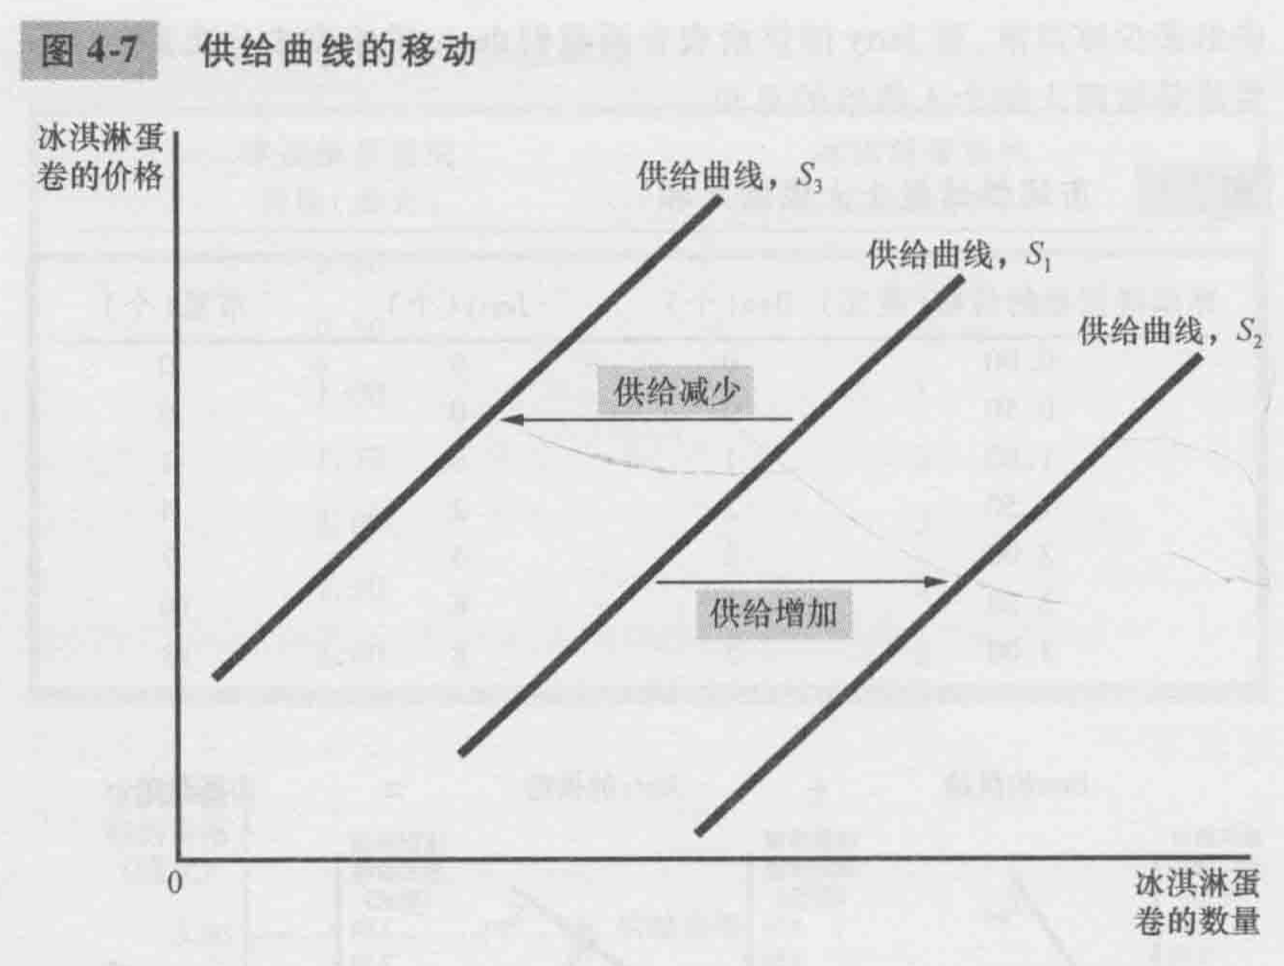
\includegraphics[width=8cm]{attachment/Fig4_7.png}
\end{figure}

与供给曲线移动相关的量: 成本, 技术, 预期, 相关激励等. 

3. 市场的需求曲线与供给曲线: 实际上, 每个消费者/生产者对价格的变化并不一定敏感, 因此个人需求/供给曲线不一定是一条直线. 然而, 由于市场上存在大量消费者/生产者, 可以认为市场的需求/供给曲线是光滑的. 

\subsection{市场均衡}

将(市场)供给曲线与需求曲线画在一张图上. 当供给曲线与需求曲线相交的时候, 就称达到了\textit{均衡}. 当供给大于需求时, 称为\textit{过剩}. 需求大于供给时, 称为\textit{短缺}. 当市场处于不均衡的状态时, 例如过剩, 此时生产者有货物积压, 他们自然地会降低价格以将货物售出, 于是逐渐达到均衡状态. 这被称作\textit{供求定理}. 另外, 我们稍后会具体分析, 为什么均衡能使得消费者和生产者的利益同时最大化. 



\subsection{弹性}

现在我们对于供给和需求的\textit{弹性}进行研究, 通俗地说就是数量随价格的变化程度, 也即线性曲线的倾斜程度. 弹性是一个相对的说法, 称某种物品的需求(供给)是\textit{富有弹性的}, 如果需求(供给)量随价格的变化较大, 反之则为\textit{缺乏弹性的}. 

\paragraph{需求价格弹性}

1. 需求价格弹性的影响因素:

\begin{itemize}
	\item 相近替代品的可获得性. 平替较多的物品一般富有弹性. 
	\item 必需品与奢侈品. 例如,正餐的弹性较低,而零食的弹性较高. 
	\item 时间范围. 例如, 在提高汽油价格的短期内汽油需求价格弹性较低, 而长期之后会有更多人购买新能源车, 因此弹性较高. 
\end{itemize}

2. 需求价格弹性的计算: 考虑$A(P_1,Q_1),B(P_2,Q_2)$, 如果直接用$E=\dfrac{\Delta Q \cdot Q^{-1}}{\Delta P \cdot P^{-1}}$(即需求量变动比率与价格变动比率之比)进行计算, 容易发现从$A$到$B$的需求价格弹性为$\dfrac{(Q_2-Q_1) \cdot Q_1^{-1}}{(P_2-P_1) \cdot P_1^{-1}}$, 显然与从$B$到$A$的需求价格弹性不同. 为此, 我们倾向于将$Q^{-1}$替换为算术平均值$\left( \dfrac{Q_1+Q_2}{2} \right)^{-1}$(实际上用其他平均值也可以). 这样的计算方法称作\textit{中点法}. 特别地, 在某一点$(P,D(P))$处的需求价格弹性为$E(P)=\lim\limits_{\delta \to 0} \left( \dfrac{D(P+\delta)-D(P)}{\delta} \cdot \dfrac{P+\frac{\delta}{2}}{D(P)+\frac{\delta}{2}} \right) = \dfrac{P}{D(P)} \cdot D'(P)$. 若定义采用其他平均值, 这里的计算结果应该是一样的. 这种算法可以快速判断一条线性需求曲线的需求价格弹性变化: 每一点的导数值相等, 那么随着$P$从$0$开始增大, $\dfrac{P}{D(P)} = \dfrac{P}{aP+c} = \dfrac{1}{a+\frac{c}{P}}$从$0$开始增大, 即弹性(的绝对值)从$0$开始增大. 

3. 各种需求曲线: 其中, 考虑针对于$\dfrac{P}{D(P)} \cdot D'(P)=E$的通解$D(P)=kP^{E}$, 需要注意需求价格弹性为负. 

\begin{figure}[H]
	\centering
	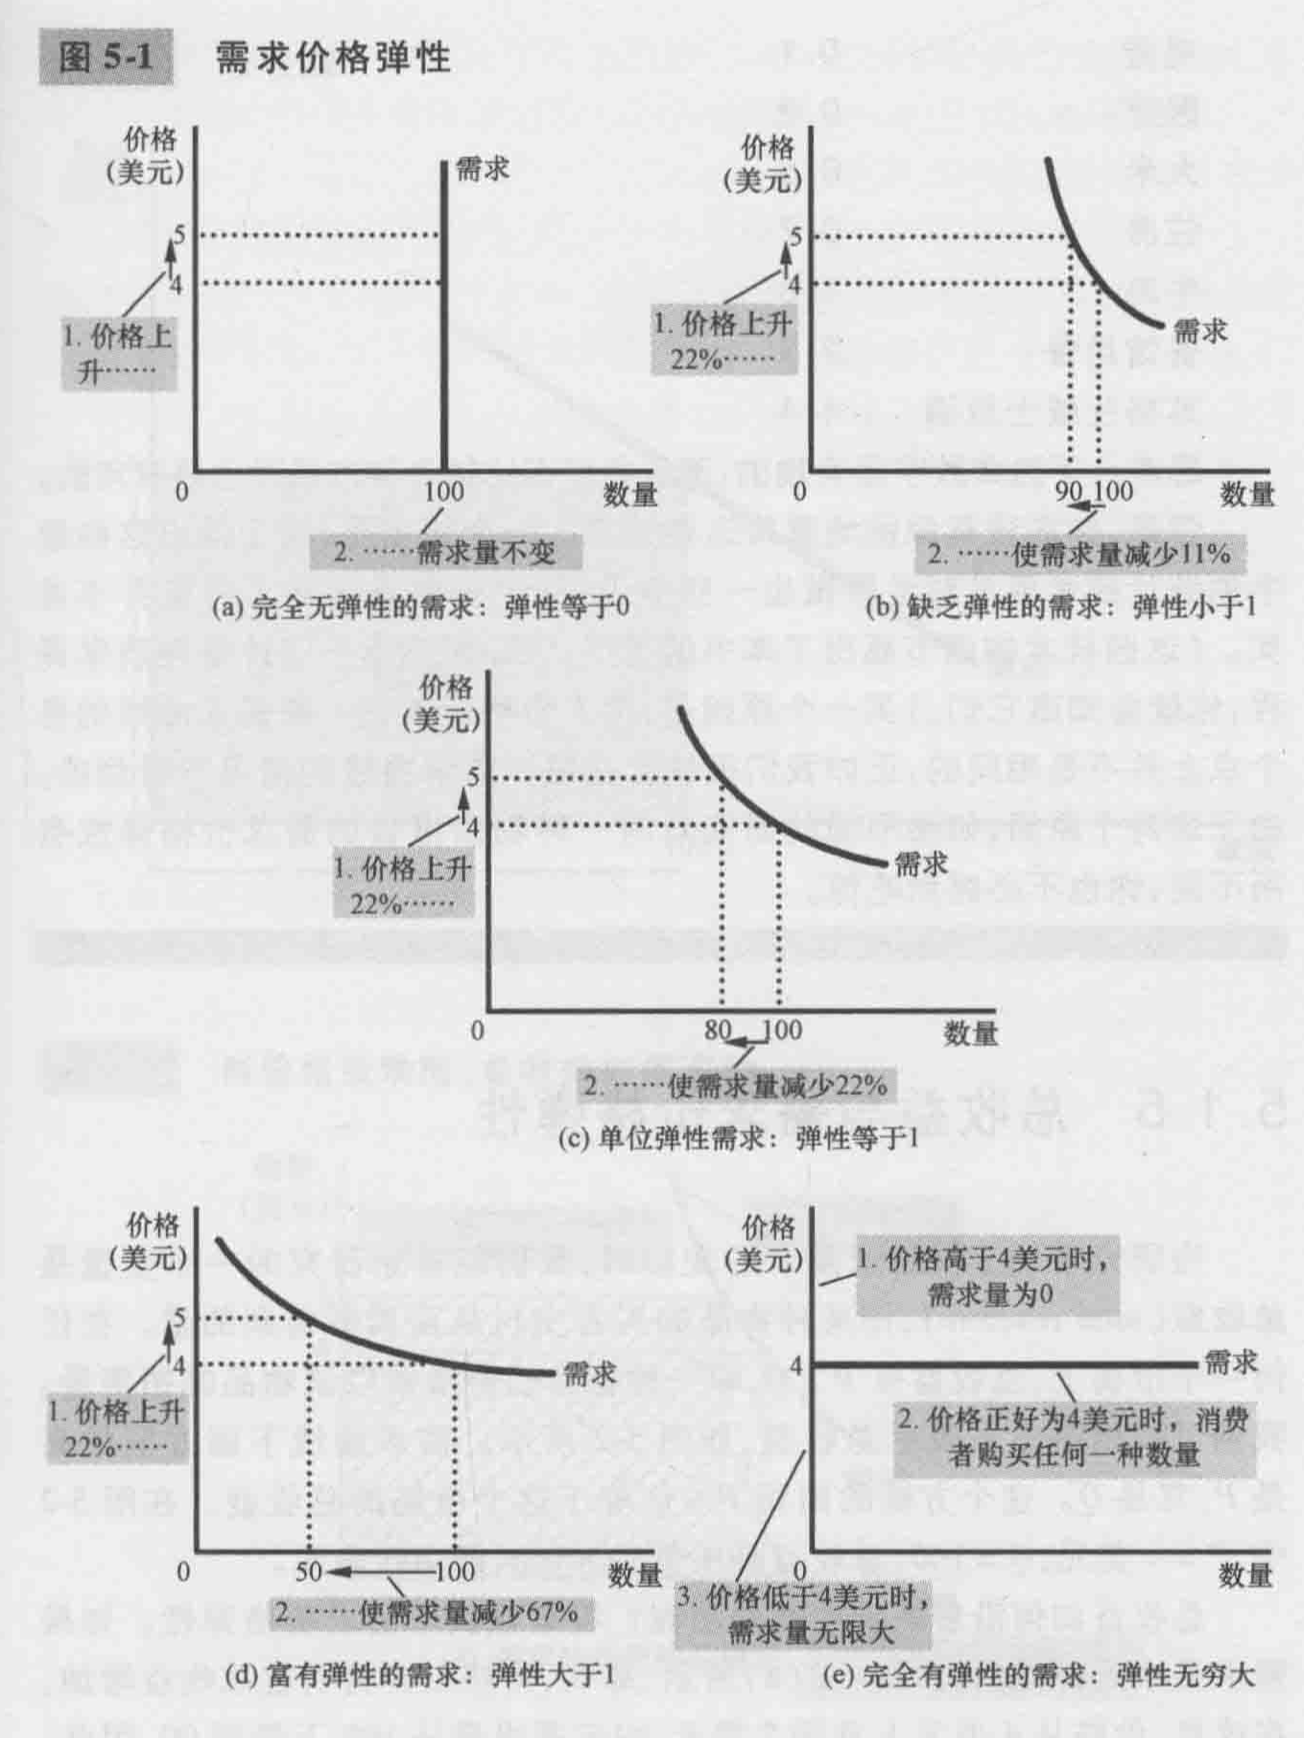
\includegraphics[width=11cm]{attachment/Fig5_1.png}
\end{figure}

4. 收益与弹性: 收益$R(P)$可以通过$P\cdot D(P)$进行计算. 我们好奇收益与弹性的关系. 直观上, 富有弹性的需求在$P$增加时会导致$D(P)$更为大幅的下降, 故$R$会减少, 反之亦然. 通过具体计算也可以说明, 以$D(P)=kP^{E}$为例, $R(P+\delta)-R(P)=k(P+\delta)^{E+1}-kP^{E+1}$. 当$E=-1$时该式为定值, 当$E>-1$时该式为正, 当$E<-1$时该式为负. 

\begin{example}{农业技术发展的影响}
	随着农业技术的发展, 相同价格下的供给量会增加(进而均衡价格下降), 然而由于农产品一般是缺乏弹性的, 这样做会使得农业市场的总收益下降, 让更多人离开农业. 
\end{example}

\paragraph{供给价格弹性}

1. 供给价格弹性的影响因素: 主要为所生产物品的灵活性, 例如不同类型流水线之间相互转换的时间成本. 这一点很容易受到时间影响. 

\begin{example}{企业的供给价格弹性}
	由于企业的生产能力通常有一个最大值, 所以在供给量低时, 供给弹性会非常高, 而在供给量高时, 供给弹性又会非常低. 体现在图像上就是上凸状(注意是数量关于价格的函数). 
\end{example}

\begin{example}{油价上升的后果}
	短期内石油的供给缺乏弹性, 因为现有的开采能力不能立刻改变; 需求也缺乏弹性, 因为消费者不会立即更换出行方式. 然而长期中供给和需求都更加富有弹性. 这就导致提高油价只能得到短期的更高收益, 同时损害了消费者的利益. 
\end{example}

2. 各种供给曲线: 由于供给价格弹性和需求价格弹性的计算方式完全一样, 我们可以直接将通解$S(P)=kP^{E}$套入. 

\begin{figure}[H]
	\centering
	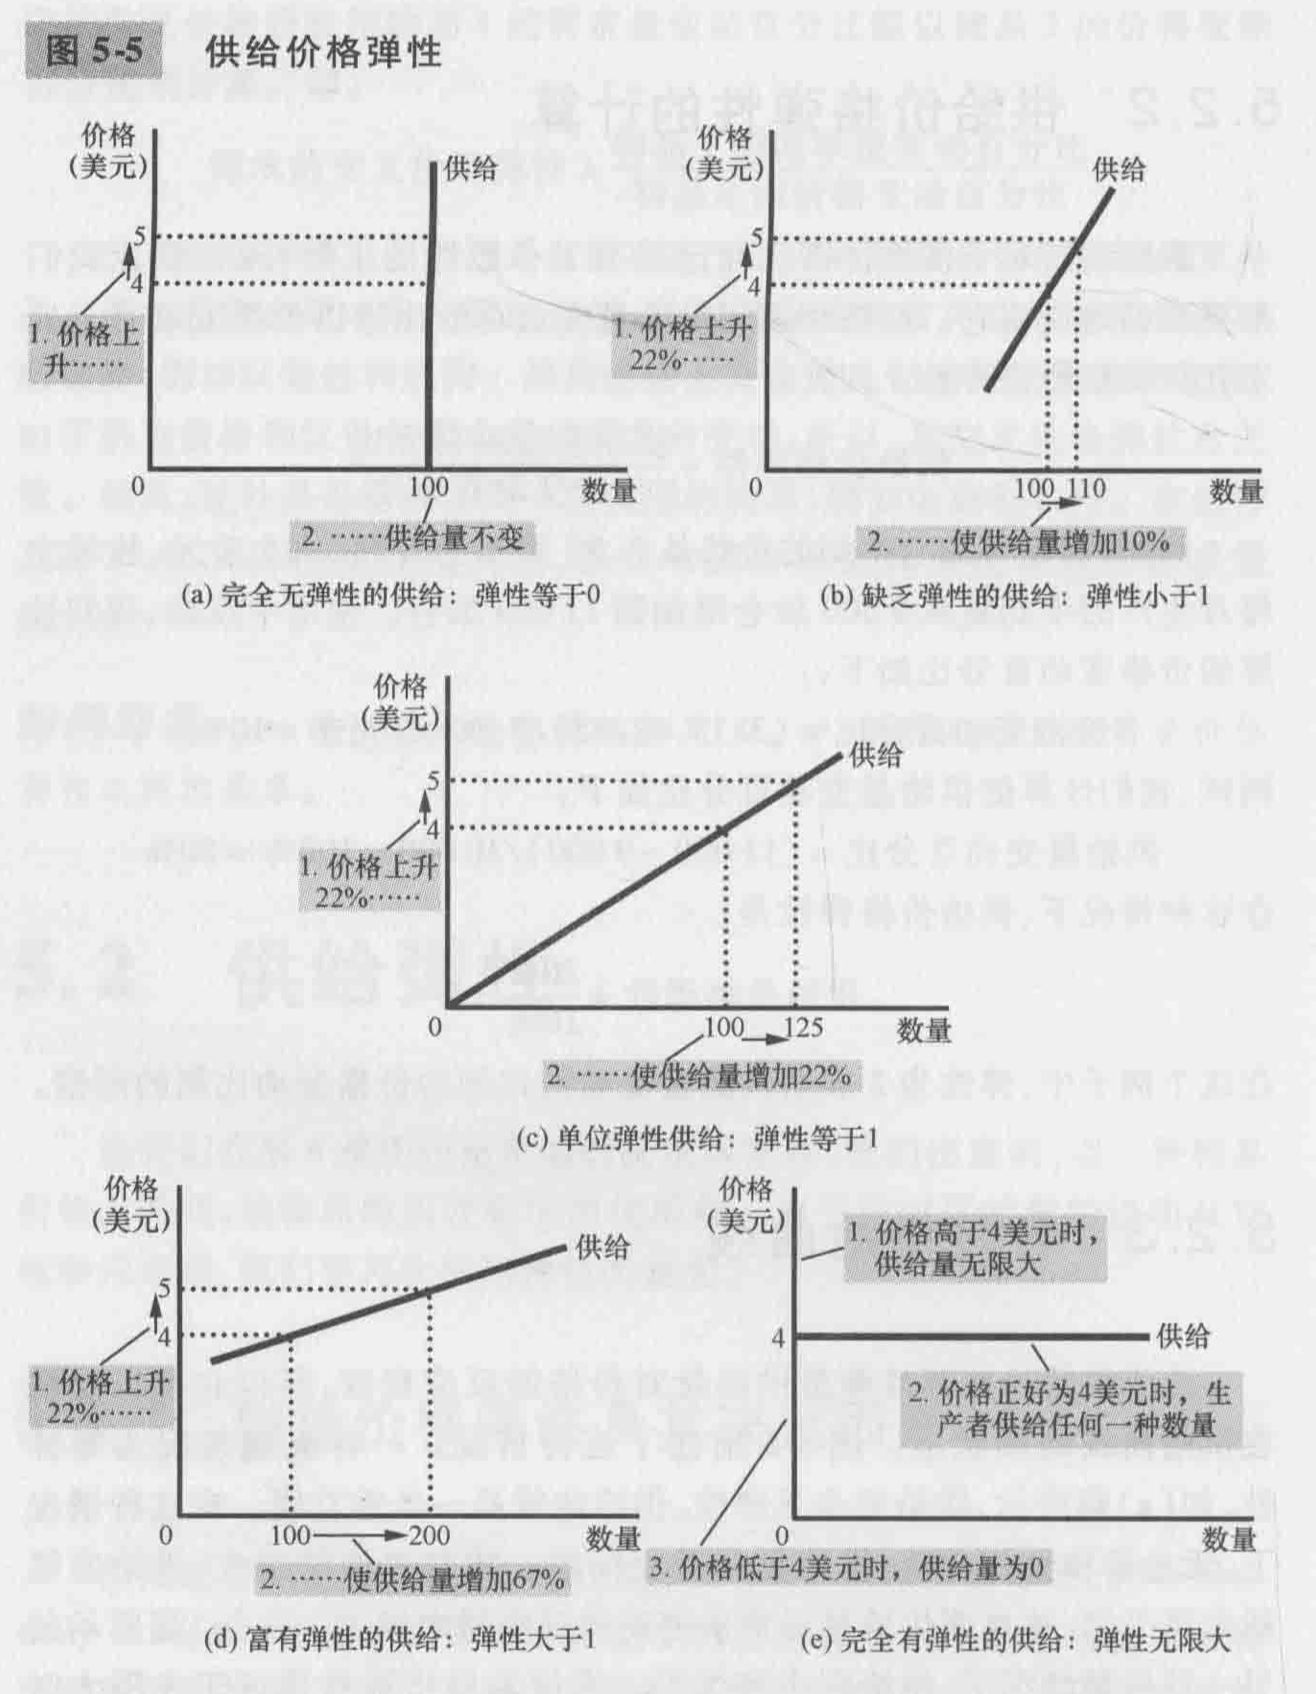
\includegraphics[width=11cm]{attachment/Fig5_5.png}
\end{figure}

\newpage
\section{福利与市场效率}

还记得之前说的经济学十大原理之一——“市场能让所有人变得更好”吗? 市场总是倾向于达成均衡状态. 如果单纯用收益(价格$\times$数量)来衡量均衡状态, 也许会发现均衡并不一定就能让收益最大化. 但另一方面, 这种算法只是站在生产者的角度, 并没有考虑消费者的利益. 类似于比较优势, 我们需要找到一种同时衡量两者获益的方法. 

先从有限情况下举例. 

考虑一个冰淇淋市场: 不同的人对价格的期望是不同的. 如果某人的支付意愿(即可以容忍的最高价格)为5美元, 而一只冰淇淋售卖价格为3美元, 那么他相当于赚到了这2美元的\textit{消费者剩余}. 类似地, 生产冰淇淋的厂家会因为技术等原因具有不同的成本, 如果某厂家的成本为2美元, 那么对于3美元的冰淇淋来说, 该厂家就赚到了1美元的\textit{生产者剩余}. 再考虑把所有人不同的支付意愿和成本综合在一起, 就能得到需求/供给曲线: 以需求曲线为例,假设$A_1,\cdots ,A_n$所对应的支付意愿为$0<P_1 \leq \cdots \leq P_n$, 那么在$0<P \leq P_1$时所有人都会付钱, 在$P_1<P \leq P_2$时除了$A_1$都会付钱……以此类推, 我们可以得到下图: 

\begin{figure}[H]
	\centering
	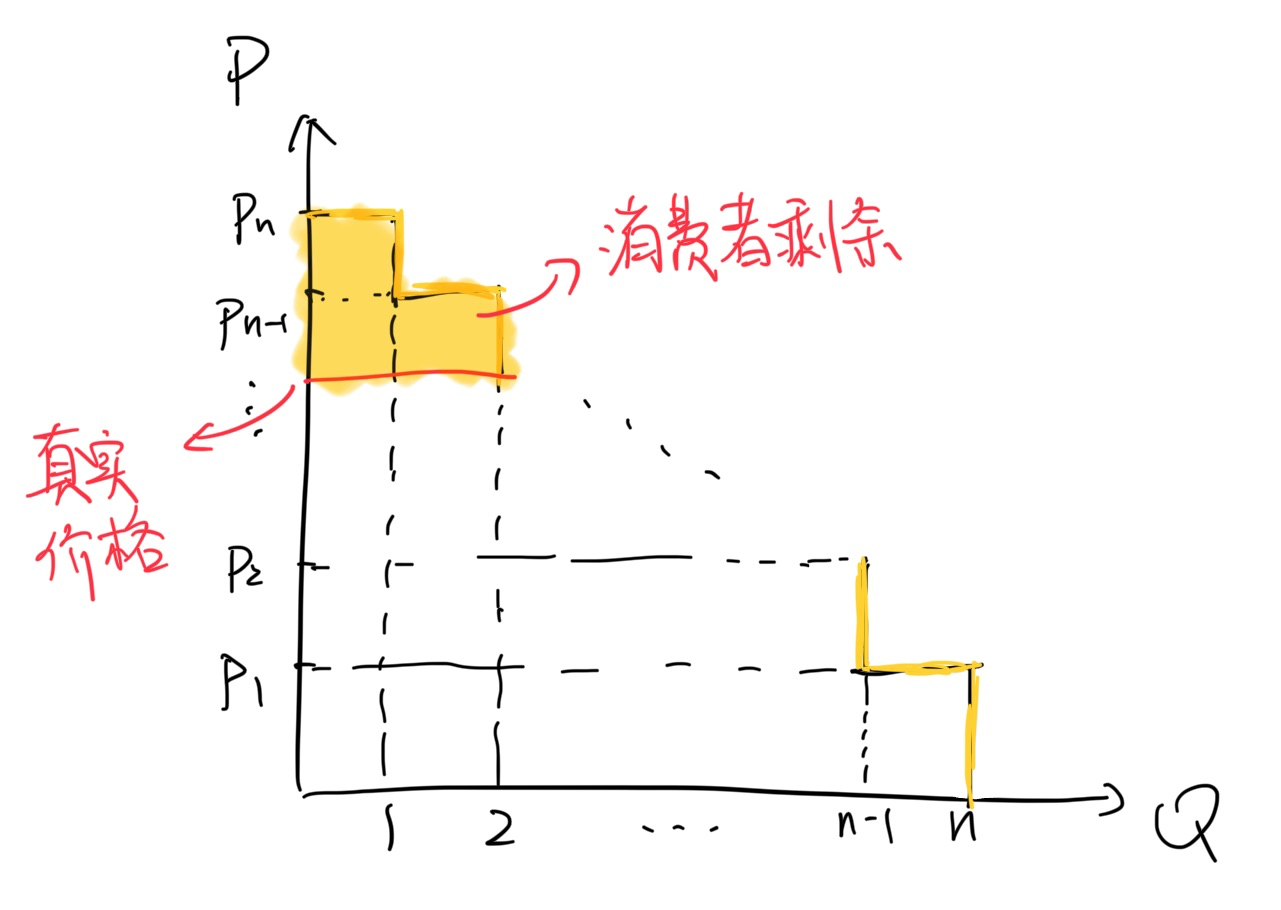
\includegraphics[width=8cm]{attachment/image-20231125092517427.png}
\end{figure}

容易发现, $0<Q\leq 1$与$P_{实} < P \leq P_n$所围成的区域刚好就是$A_n$的消费者剩余. 类似地可以得到: 需求曲线与真实价格所围成的区域面积就是消费者总剩余. 

生产者剩余也是同样的. 容易得到: 供给曲线与真实价格所围成的区域面积就是生产者总剩余. 

通过简单的推导, 不难得到下面结论: 

1. 市场将供给分配给对这种商品评价最高的消费者, 将需求分配给成本最低的生产者. 

2. 均衡状态能使消费者和生产者的利益最大化: 由于消费者剩余$=$买者总评价$-$买者支付, 生产者剩余$=$生产者收益$-$生产者总成本, 将它们加和即得: 总剩余$=$买者总评价$-$生产者总成本. 在价格高于均衡价格时, 降低价格则意味着减少卖者成本并增加买者评价, 这会导致总剩余上升; 价格低于均衡价格时同理. 

\begin{figure}[H]
	\centering
	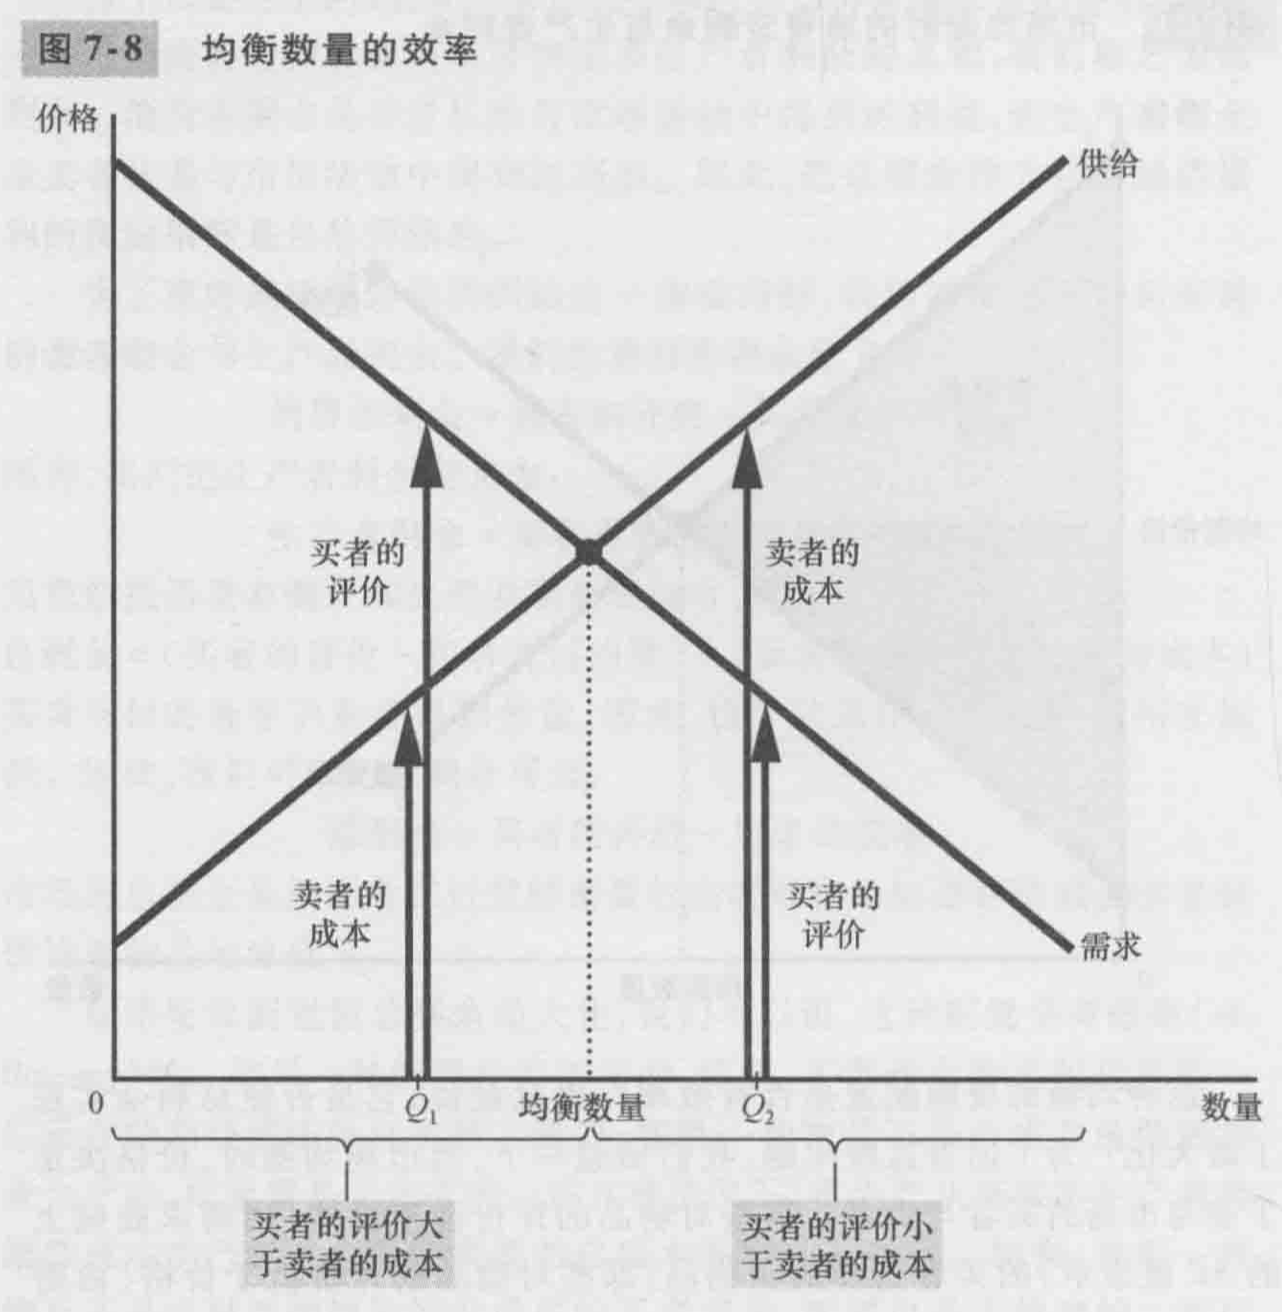
\includegraphics[width=8cm]{attachment/Fig7_8.png}
\end{figure}

下面用三个例子来阐释市场剩余的分析思路. 

\subsection{价格控制}

之前提到过, 政府面临效率与平等的权衡. 例如对于租房市场, 为了让穷人也有地方住, 政府会给定一个价格上限. 如果价格上限高于均衡价格, 相当于没有影响; 但该上限常常低于均衡价格, 此时在价格触及上限后不能再上升, 就会导致短缺. 尝试用剩余的方法衡量谁的利益受损: 

\begin{figure}[H]
	\centering
	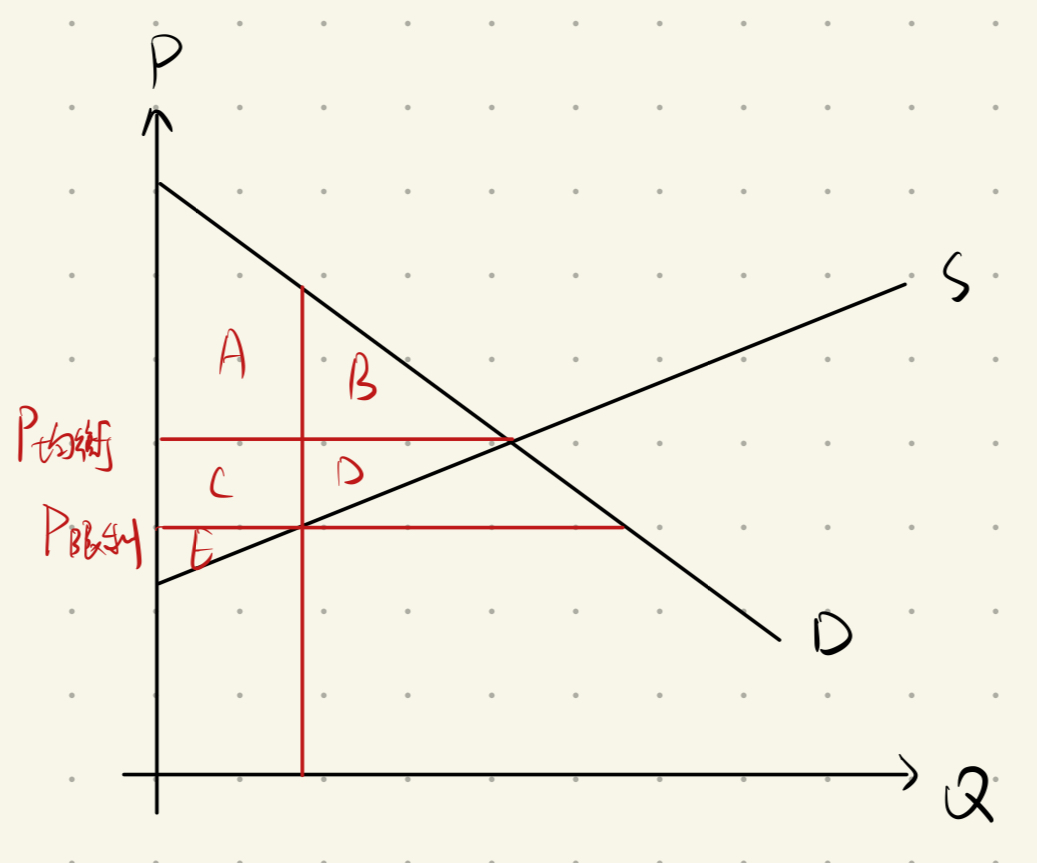
\includegraphics[width=8cm]{attachment/IMG_3835.jpg}
\end{figure}

不难发现, 消费者剩余从$A+B$变成了$A+C$(增加还是减少取决于具体的价格限制), 生产者剩余从$C+D+E$下降至$E$, 而总剩余从$A+B+C+D+E$下降至$A+C+E$. 这里称由于市场扭曲导致的损失为\textit{无谓损失}, 即图中的$B+D$. 

无谓损失的最终来源, 是高于限制价格时潜在的交易好处. 

\subsection{税收}

首先讨论\textit{税收归宿}的问题, 即税收应当如何在消费者与生产者之间分配. 容易发现, 向消费者征税和向生产者征税是完全一样的(都会导致需求曲线与供给曲线的相对差距缩小, 且缩小量相同). 因此, 可以把税收想象为打入生产者得到的价格与消费者提供的价格间的楔子. 

\begin{figure}[H]
	\centering
	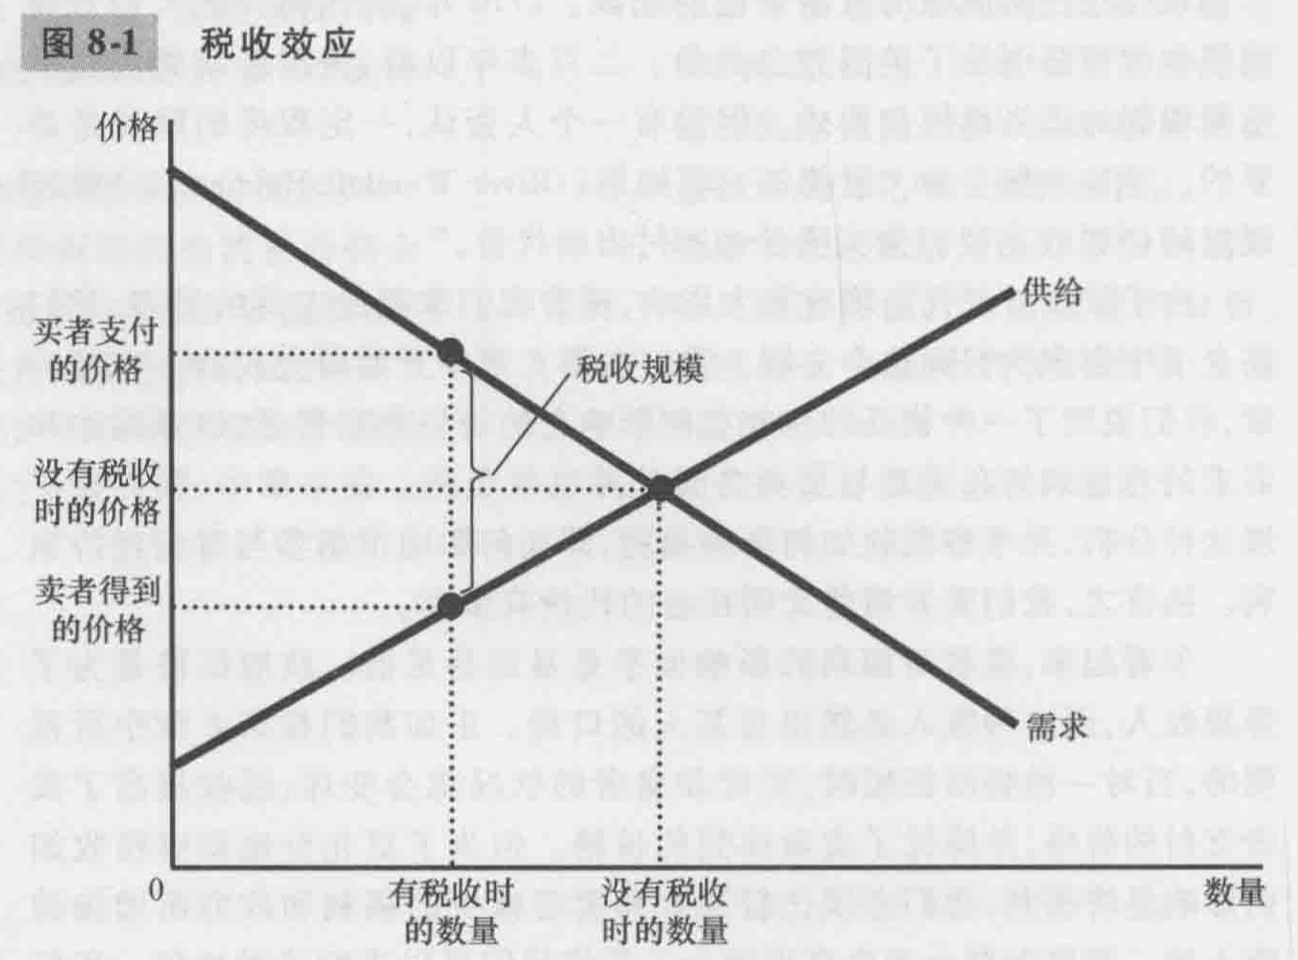
\includegraphics[width=9cm]{attachment/Fig8_1.png}
\end{figure}

从上图可以看出, 税收在消费者和生产者之间按照其弹性成比例分配. 

接着用剩余工具分析税收的无谓损失: 

\begin{figure}[H]
	\centering
	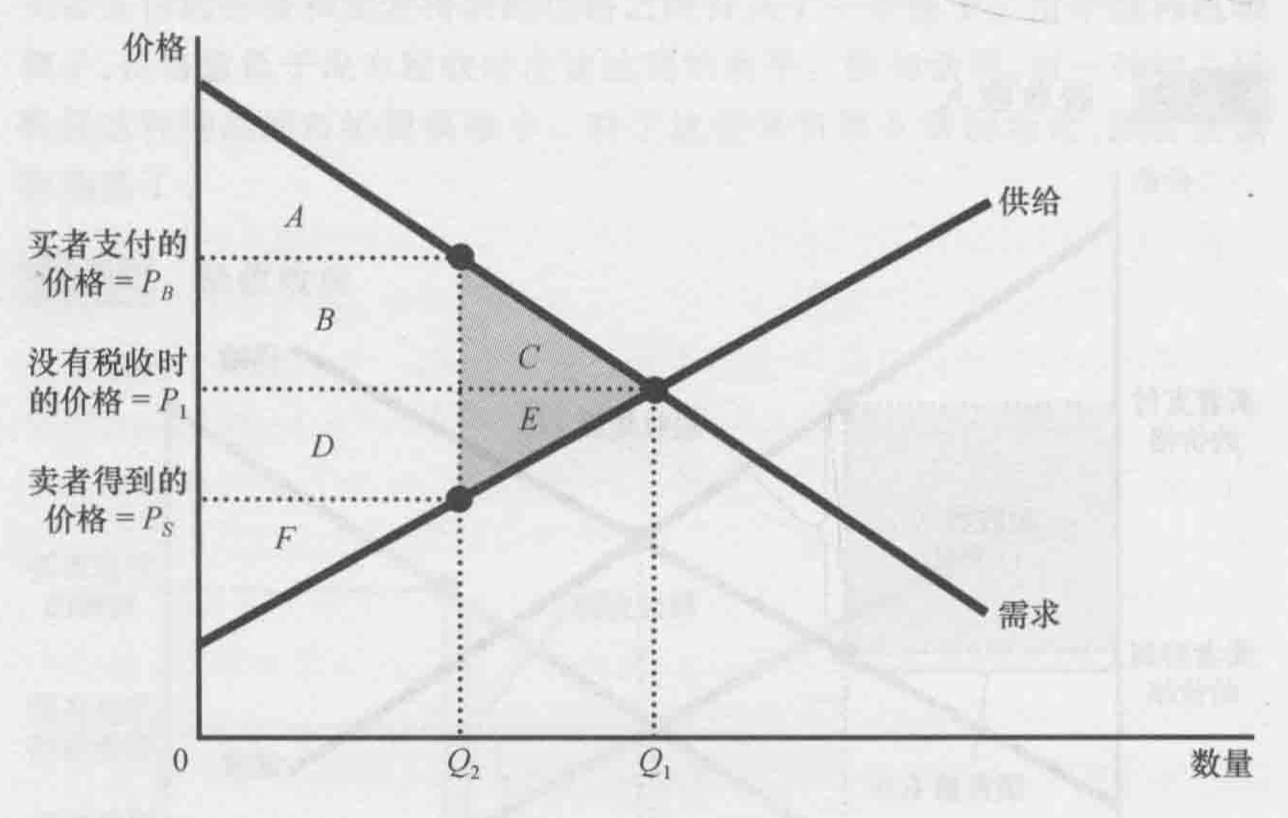
\includegraphics[width=9cm]{attachment/Fig8_3.png}
\end{figure}

消费者剩余减少了$B+C$, 生产者剩余减少了$D+E$, 但是税收提供的额外收入只有$B+D$, 这说明税收的无谓损失就是$C+E$. 

从图中也能看出, 随着税收的增加(即$Q_2$向左移动), 税收收入$B+D$会先增大再减小, 因此有时增加税收反而会减少税收收入. 另外, 税收带来的无谓损失会一直增加. 

\subsection{国际贸易}

这里, 我们总是假设一个国家相对整个世界市场而言是\textit{价格接受者}, 即它的市场行为不会影响世界价格. 或者说, 可以将世界价格视作一个弹性为$0$的需求/供给. 

\begin{figure}[H]
	\centering
	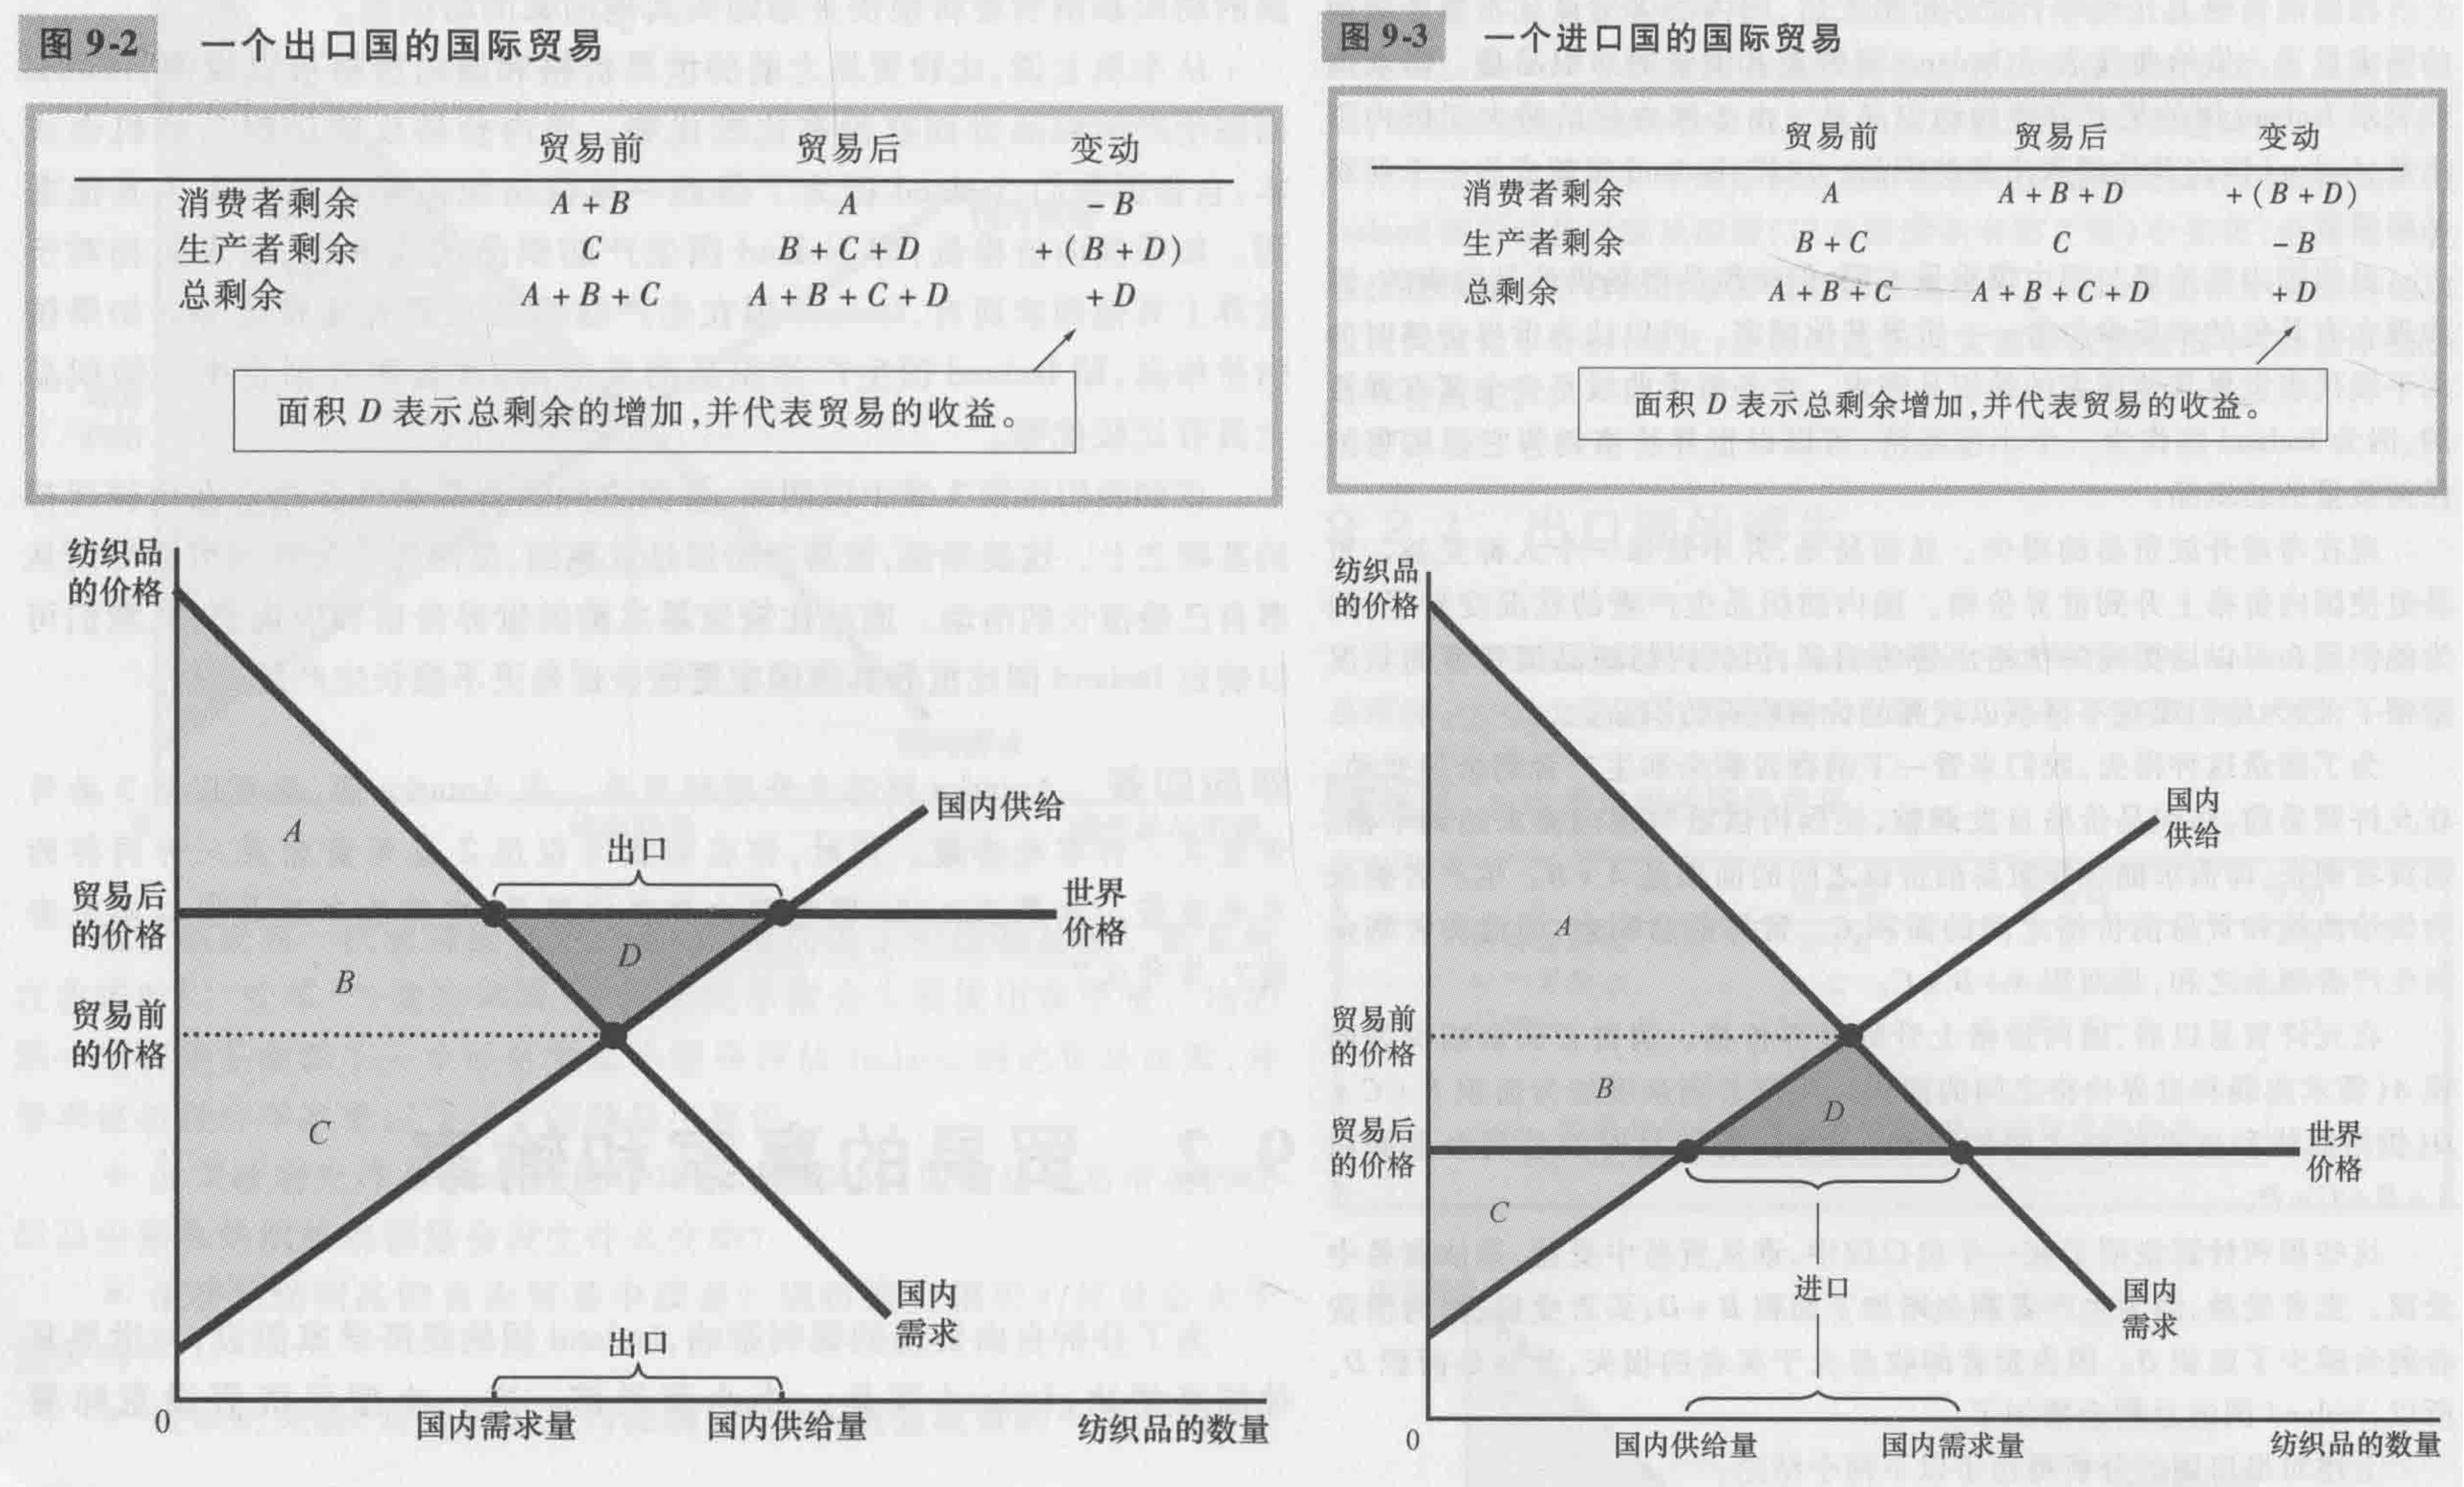
\includegraphics[width=18cm]{attachment/Fig9_2,3.png}
\end{figure}

出于各种原因, 一国政府常常对进口物品征收关税. 下面来分析关税的影响: 

\begin{figure}[H]
	\centering
	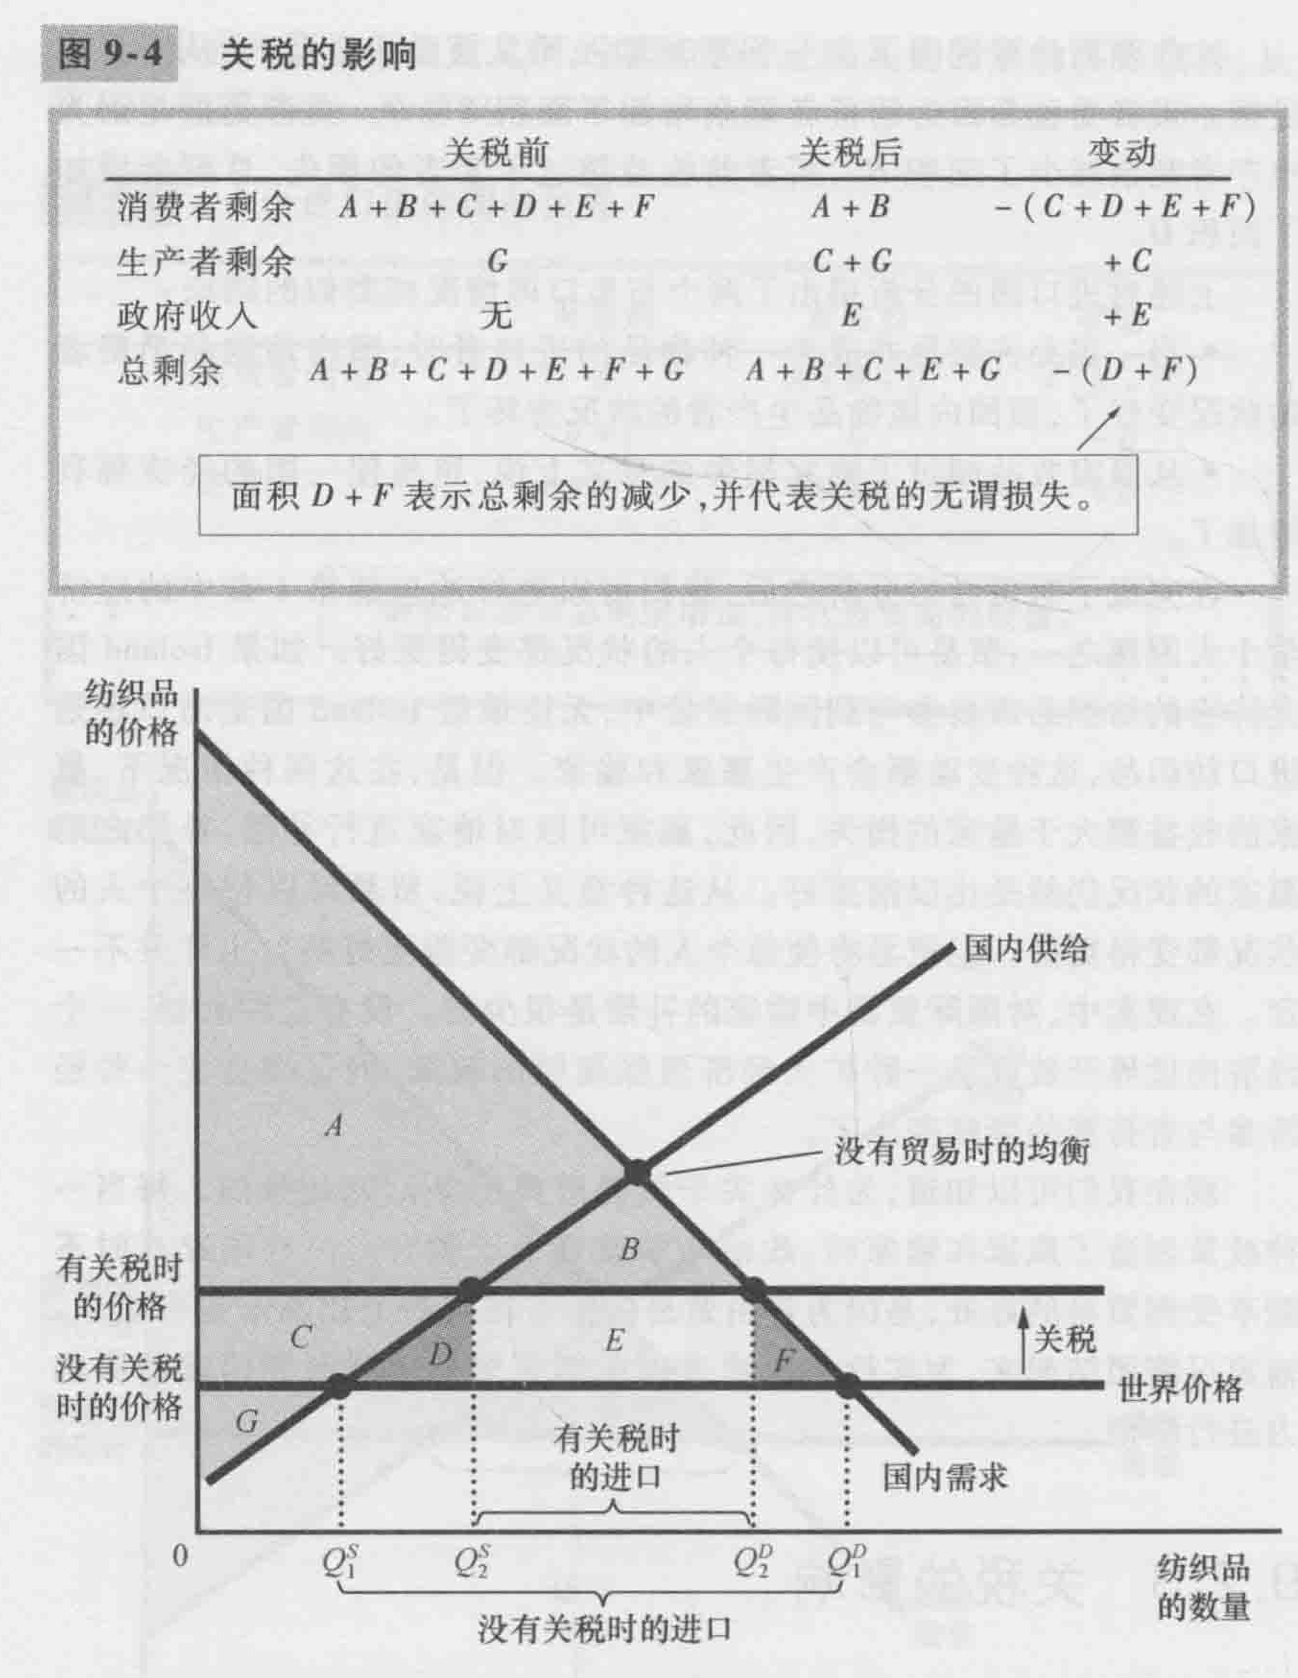
\includegraphics[width=9cm]{attachment/Fig9_4.png}
\end{figure}







